\documentclass[letterpaper,10pt,conference]{ieeeconf}   % Use this line for a4 paper
\usepackage{fancyhdr}
\usepackage{graphicx}
\usepackage{amssymb}
\usepackage{epstopdf}
\usepackage{amsmath}
\usepackage{amssymb}
\usepackage{cite}
\usepackage{float}
\usepackage[normalem]{ulem}
\usepackage{multirow}
\usepackage{booktabs} 
\usepackage{wrapfig}
\usepackage{caption}
\usepackage[aboveskip=2pt]{subcaption}
\usepackage[linecolor=black,backgroundcolor=lightgray]{todonotes}
\usepackage[colorlinks=true, linkcolor=black,citecolor=black,urlcolor=blue]{hyperref}
\DeclareGraphicsRule{.tif}{png}{.png}{`convert #1 `dirname #1`/`basename #1 .tif`.png}
\setlength{\abovecaptionskip}{2pt} % Chosen fairly arbitrarily
\pdfminorversion=4

\IEEEoverridecommandlockouts               % This command is only needed if 
                             % you want to use the \thanks command
                             
\overrideIEEEmargins                   % Needed to meet printer requirements.

\hyphenation{op-tical net-works semi-conduc-tor}

%\pagestyle{fancyplain}
%\topmargin =-30pt
%\lhead{ \footnotesize {\textit{Submitted to:} The 2018 American Control Conference – ACC 2017 - Due 09/25/17}}
%\rhead{ \footnotesize {\textit{Final} -- \today}}
%\headsep=25pt


%%%%%%%%%%%%%%%%%%%%%%%%%%%%%%%%%%%%%%%%%%%%%%%%%%%%%%%%%%%%%%%%%%%%%%%%%%%%%%%%%%
%%%%%%%%%%%%%%%%%%%%%%%%%%%%%%%%%%%%%%%%%%%%%%%%%%%%%%%%%%%%%%%%%%%%%%%%%%%%%%%%%%
\begin{document}
\title{\LARGE \bf Modeling and Control of a Flexible Catheter for Cardiac Ablation}

\author{Daniel Newman$^{1}$, Charles Taylor$^{1}$, and Joshua Vaughan$^{1}$% <-this % stops a space
\thanks{$^{1}$Department of Mechanical Engineering,
        University of Louisiana at Lafayette, Lafayette, Louisiana 70504 USA
        {\tt\small joshua.vaughan@louisiana.edu}}%
}

    
% make the title area
\maketitle

% As a general rule, do not put math, special symbols or citations
% in the abstract
\begin{abstract}
The control of human-operated flexible systems is a problem that has generated significant research. A variety of methods have been proposed to eliminate disturbances to flexible systems. By simplifying disturbances by representing them as impulses that generate initial conditions, some researchers have used impulse-based command generation to reduce existing vibration. This approach closely resembles the common open-loop input shaping method. However, existing literature does not thoroughly account for robustness requirements. This paper expands on the concept of initial condition input shaping and proposes a method of providing robustness to variations in natural frequency. The concept of Specified Insensitivity is used to generate these robust input shapers. Experimental results are provided which support these findings.
\end{abstract}

% creates the second title. It will be ignored for other modes.
%\IEEEpeerreviewmaketitle

\section{Introduction}
\label{sec:intro}

In this review, the basics of atrial fibrillation and its clinical interventions are discussed. First, this section will establish the basics of cardiovascular physiology, particularly as it pertains to the left atrium. Mechanisms of atrial fibrillation will also be introduced. Next, Section \ref{sec:diagnosisandmanagement} will discuss some risk factors of atrial fibrillation and typical diagnosis and management with clinical drugs. Section \ref{sec:ablation} will introduce the topic of cardiac ablation as an intervention technique and describe the general procedure. Current technology, including various control equipment and its FDA classifications will be discussed in Section \ref{sec:currenttech}. Finally, Section \ref{sec:research} will address current advances in robotic technology that are both being used in clinical practice and developed in academic research.

The human heart is comprised of four chambers - the left and right atria and the left and right ventricles. Deoxygenated blood flows through the superior and inferior vena cavae into the right atrium, where it is pumped through the tricuspid valve into the right ventricle. Then, it leaves the right ventricle through the aortic valve and passes through the lungs where it receives oxygen through diffusion. After leaving the lungs, oxygen-rich blood enters the left atrium, passes through the mitral valve into the left ventricle and into the pulmonary artery and aorta through the pulmonary valve. After leaving the heart, the oxygen-rich blood passes through the body and returns through the great veins to begin the process once more. 

The cardiac cycle is governed by electrical impulses intrinsic to the cardiovascular cells. When exposed to electrical excitation, all muscular heart tissue will exhibit regular contraction. This beating is orchestrated by modified cells called myocytes. In nominal heart function, a specific region of the right atrium possesses a bundle of myocytes called the Sino-atrial node. This region is colloquially referred to as the ``pacemaker'', because its discharge initiates the cascading excitation of the heartbeat. The electrical impulse from the Sino atrial node passes through the atrioventricular node into the Bundle of His across the heart. 

Because each cell in the heart has similar electrophysiology, it is accurate to say that any such cell has the potential to be a ``pacemaker.'' However, the Sino-atrial node generally possesses the highest frequency of excitation, and therefore dominates the rate of discharge. When anomalies occur in the rate of excitation of the atrial myocytes, they can cause atrial fibrillation. 

Atrial fibrillation is a condition where normal heart rhythm is compromised by inappropriate firing of atrial myocytes. When atrial fibrillation occurs, the electrocardiogram of the patient exhibits obvious, abnormal characteristics. In nominal heart function, the first electrical event is called the “P” wave, which indicates atrial excitation. When atrial fibrillation occurs, this wave becomes less regular, resulting in less effective ventricle excitation.

%%%%%%%%%%%%%%%%%%%%%%%%%%%%%%%%%%%%%%%%%%%%%%%%%%%%%%%%%%%%%%%%%%%%%%%%%%%%%%%%%%
%%%%%%%%%%%%%%%%%%%%%%%%%%%%%%%%%%%%%%%%%%%%%%%%%%%%%%%%%%%%%%%%%%%%%%%%%%%%%%%%%%
\section{Atrial fibrillation diagnosis and management}
\label{sec:diagnosisandmanagement}

Although not inherently dangerous, atrial fibrillation carries increased risk of a number of health complications such as stroke. Atrial fibrillation can be paroxysmal, persistent or permanent.  Although rare in the general population, its occurrence is $5-15\%$ in 80 year olds. The varying seriousness of this condition results in a number of intervention approaches based on the need.

When first diagnosed with atrial fibrillation, a 12-Lead electrocardiogram is performed on the patient to accurately map the electrophysiological function. Depending on the diagnosed risk of stroke or acute heart failure, the patient may require cardioversion and anticoagulants.  A number of factors need to be taken into account when identifying risk of stroke, including age, gender, and history of other conditions \cite{lip:10a}.

Because stroke is the primary risk of atrial fibrillation, an important aspect of managing this condition is antithrombotic management. Low risk patients are often instructed to take asprin \cite{camm:10a}, while higher risk patients are prescribed other oral anticoagulants such as a Vitamin K antagonist. Clinical studies have strongly demonstrated the efficacy of antithrombotic therapy as a deterrent against stroke \cite{hart:07a}. Beyond these measures, drugs which control the rate and rhythm of the heart can be taken. In this regard, both approaches are viewed as equally effective at preventing death due to cardiovascular complications \cite{camm:10a,atrial:02a,van:02a}.   

\section{Cardiac ablation}
\label{sec:ablation}

If atrial fibrillation cannot be effectively managed by the litany of available medications, catheter ablation has been shown to provide long-term relief from symptoms. The current guidance on performing catheter ablation is that the patient should have attempted to manage their symptoms with at least one medication before considering surgical intervention \cite{camm:10a}. Furthermore, rigorous scientific studies have thus-far only focused on the efficacy of ablation to manage proximal atrial fibrillation. Some clinicians have advocated for its use as a primary intervention technique due to its success in eliminating arrhythmia caused by atrial fibrillation. 

Cardiac ablation therapy as a treatment for atrial fibrillation dates back into the 1990's as part of open heart surgery \cite{cox:91a}. Overall, some literature reviews indicate the superiority of radiofrequency ablation in comparison to anti-arrhythmic drugs \cite{cappato:05a,calkins:09a}. One limitation mentioned in this meta-analysis is the fact that relatively few centers are performing this intervention. Therefore, applicability into standard clinical practice is questionable. One review evaluates the efficacy of cardiac ablation in its ability to relieve symptoms of paroxymal atrial fibrillation over a long period of time \cite{cheema2006long}. This review indicates that long-term success resulting from a single procedure is less than $40\%$, and points to limitations in the follow-up of patients after the procedure. Many clinical studies do not follow up with patients after one year following the procedure.  

While a predominant strategy in catheter ablation is to isolate the left atrium from the pulmonary veins, this is likely not a guaranteed way to manage atrial fibrillation for all patients. One study \cite{nademanee:04a} demonstrated that mapping the cardiovascular substrate provided clinicians with good information on which sites to target for ablation. The authors of this study specifically note that many patients ``may not have benefited from solely the pulmonary vein isolation technique.'' 

\subsection{Representative Intervention}
\label{sec:repintervention}

The procedure for catheter ablation can differ by clinician, but several aspects of the intervention are consistent. In ablative surgery, the surgeon makes an incision near the groin to facilitate insertion of a catheter into the inferior vena cava. From here, the catheter is navigated through the great vein into the right atrium. Because atrial fibrillation typically originates from irregular electrical signals in the pulmonary veins, the catheter is navigated into the left atrium. This is typically done by performing a transseptal puncture. Next, the left atrium is mapped by magnetic imaging. This mapping will give the clinician information on electrophysiological abnormalities of the patient. With this information, a catheter with a radiofrequency-emitting end effector is navigated to the desired regions. The abnormal tissue is ablated, thereby eliminating the flow of the undesired electric current. 


\section{Current technology}
\label{sec:currenttech}

Currently, a variety of tools are on the market for performing ablative cardiac surgery. The FDA has several classifications for the devices marketed by these manufacturers. Generally, they all fall under Section 870 - Cardiovascular Devices \cite{FDA:870}. First, Section 870.1220 identifies ``Electrode Recording Catheter or Electrode Recording Probe'' devices \cite{FDA:870.1220}. These devices are classified as Type II products. An example is the Biosense Webster Lasso Circular Mapping Catheter \cite{BiosenseWebster:Lasso2515}.  Next, the ablative catheters used to perform the surgical procedure are regulated as Type III devices. The regulatory definition of these devices from the FDA is, ``an ablation catheter that features electrodes through which thermal energy is delivered \cite{FDA:OAD}.'' Boston Scientific manufactures a representative device under this classification, called the Blazer II \cite{BostonScientific:BlazerII}. Finally, Section 870.5700 outlines the guidance on "steerable cardiac ablation catheter remote control systems \cite{FDA:870.5700}." 

Ablative catheter technology is continuing to improve. A recent example of this is the FDA approval of Biosense Webster's Thermocool SmartTouch catheter \cite{BioSenseWebster:FDAApproval}. This device has force sensing on the ablative tip, allowing clinicians to determine precisely what force is being exerted on the cardiac tissue during ablation. Using this Class III FDA approved device, initial studies suggest that this additional information may be useful in increasing success of ablation procedures \cite{natale:14a}.  

Although most work in catheter ablation is done on patients experiencing paroxysmal atrial fibrillation, some studies have demonstrated the efficacy of this procedure to provide relief from persisting atrial fibrillation. One such study \cite{ouyang:05a} used the Biosense Webster Thermocool NaviStar to map the electrophysiology of the left atrium. Using lasso catheters, the pulmonary veins were completely isolated from the left atrium. 

\section{Research and Development}
\label{sec:research}

A number of researchers are working to increase the productivity of surgeons in catheter ablative surgery. Some advanced robotic systems have recently been developed to provide remote control of catheter systems with various methods for providing high precision control. In general, these systems are designed to increase safety and efficiency. Safety is increased by reducing exposure of patients, clinicians, and staff to radiation by reducing exposure time due to reduced procedure duration and remote manipulation of the catheter. Typically, catheters are guided by flouroscopy, which uses X-Ray radiation to yield a real-time image of the device within the patient. Surgeons need to wear protective gloves and lead vests to protect themselves. Furthermore, efficiency is a concern for these procedures. Typically, catheter cardiac ablation is performed by highly skilled surgeons. Even still, this procedure typically takes around four hours. By providing clinicians with the tools to effectively perform this procedure with better information and more robust control over the catheter location, advanced robotic systems can theoretically shorten procedure durations.

\subsection{Automatic and semi-automatic systems}
\label{sec:autosemiauto}

A substantial amount of work is being done to investigate the use of robotics in catheter surgery \cite{rafii2014current}. One area of growth is in the simulation of surgical procedures. As technologies develop, new ways of objectively evaluating surgical skill can be used through simulations and robotic means. Next, improved technologies bring improved mapping systems. Current robotic systems utilize three-dimensional electroanatomic mapping to provide real-time information on catheter location. This technique can be incorporated with pre-operative information to provide more accurate real-time data in animal trials \cite{reddy:07a}.

One such advanced system is the NIOBE \cite{NIOBE}, which utilizes magnets to guide the catheter from remote user input. Some trials have been performed on humans to demonstrate the effectiveness and safety of this system in clinical use \cite{pappone:06a}. Preliminary data indicates that procedure duration and operator skill requirements can be lowered by using this remote robotic system. One limitation with this system is that, because it uses magnets, the NIOBE would be incompatible with some implants in patients. 

Another similar system is the SenseiRobotic Catheter System by Hansen Medical \cite{HansenMedical:Sensei}. One key difference between this system and the Niobe is that the Sensei is simply a robotic control mechanism for standard market catheters. The same premise of removing the surgeon from the operating table and allowing remote manipulation of the catheter is utilized in this system. This system has been demonstrated to be safe on humans \cite{saliba:08a} and is FDA approved as a Class II device. 

Academic research is also being conducted on providing remote manipulation of surgical catheters by various means. One group replicated the traditional catheter controls into a remotely operated robotic system \cite{thakur:09a}. Another group created a robotic catheter system with force feedback using the Phantom omni and demonstrated its use in experimental trials \cite{xiao2012robotic}. A similar teleoperated robotic device intended for neurosurgery was designed and evaluated by a small group of surgeons \cite{srimathveeravalli:10a}. A surgeon with extensive catheter experience was able to use a remote robotic system more efficiently than manual manipulation during \textit{ex-vivo} testing of an animal heart \cite{cercenelli:07a}. 


\section{Modeling}
\label{sec:modeling}

A number of researchers have analyzed the kinematics of cardiac catheters. In most cases, the primary consideration is the bending and relaxation of the curved tip. A kinematic approach based on Denavit-Hartenberg nomenclature has been developed and experimentally compared to real catheter motion \cite{ganji:09a}. Catheter behavior in the presence of nonlinearities such as friction and backlash are routinely considered \cite{hasanzadeh:17a}.

\section{Control}
\label{sec:Control}

Several research groups have created various control algorithms to interact with the clinician. In one instance, proportional-derivative control with haptic feedback was used to enable teleoperation of a catheter system \cite{srimathveeravalli:10a}. This system was evaluated by clinicians in a simulated \textit{in-vivo} environment. In another study, a robotic platform was designed to accept generic catheters and accurately position them with minimal lag \cite{thakur:09a}. 

One method of controlling the catheter involves using magnetic fields to manipulate and sense its positioning. For instance, a proposed control method utilizes embedded magnets within the catheter to control it with an external magnetic field \cite{le:16a}. This method was experimentally tested to demonstrate its capability of reaching the desired equilibrium states \textit{ex-vivo}. 

Substantial research has been performed to correctly predict the contact force of the catheter tip on a surface \cite{natale:14a}. A model-based approach to understanding the backlash and hysteretic effects of a catheter was used to approximate its contact force with the environment \cite{khoshnam:14a}. These methods were experimentally validated \textit{ex-vivo} to demonstrate the capabilities of accurate positioning and force sensing. Experimental tests further were used to track a sinusoidally varying surface with accurate force. PID control was used to bring the actual catheter deflection to its desired, user-given values.

Curiously, dynamic interactions between the ablative catheter and blood flow are widely ignored in current literature. This trend is based on the conclusion that forces resulting from blood flow are trivial compared to the dynamic interaction between the catheter and the heart wall \cite{salimi:11a}. In one study, nonlinear model predictive tracking control was developed for ablative cardiac catheters \cite{soltani:17a}. This controller considered the interaction between the cardiac wall and the the catheter, while ignoring blood flow.

%%%%%%%%%%%%%%%%%%%%%%%%%%%%%%%%%%%%%%%%%%%%%%%%%%%%%%%%%%%%%%%%%%%%%%%%%%%%%%%%%%
%%%%%%%%%%%%%%%%%%%%%%%%%%%%%%%%%%%%%%%%%%%%%%%%%%%%%%%%%%%%%%%%%%%%%%%%%%%%%%%%%%
\section{Dynamic Model}
\label{sec:intro}
%
\begin{figure}[t!] 
\begin{center}
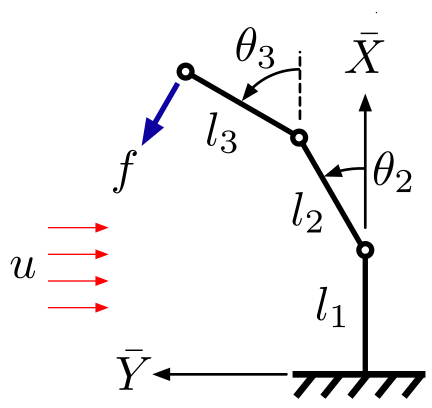
\includegraphics[width = 2.7in]{Figures/Planar_Model} 
\caption{Dynamic model of a two link flexible-arm manipulator} 
\label{fig:model}
\end{center}
\vspace{0.1in}
\end{figure}
%
The dynamic model used in this analysis is shown in Fig.~\ref{fig:model}. A flexible beam is assumed to be fixed at its base. The rotation of each element about the $\bar{Z}$-axis is designated by $\theta_{i}$, where $i$ is the element number. As depicted in this Figure, each rotation is defined relative to the global coordinate frame. The generalized coordinates are arranged in the following form:
%
\begin{equation}
\label{eq:nodaldisp}
Q_{n \times 1} = 
\begin{bmatrix}
 \theta_{1} & 
 \theta_{2} &
 \dots & 
 \theta_{n} & 
\end{bmatrix}^T.
\end{equation}
%

\subsection{System Inputs}
\label{sec:inputs}

The input to the system is given as force applied to the distal tip of the $n^{th}$ element, $f$. In addition, a known velocity field, $\vec{U}$, exerts drag forces on each element. These drag forces generate moments at each hinge, causing deflection of the catheter. These moments are given by:
%
\begin{equation}
\vec{\gamma}_{n} = \int_{0}^{l_n} \vec{r}_n(x) \times \vec{f}_n(x) \mathrm{d}x,
\end{equation}
%
where:
%
\begin{equation}
\label{eq:r_vector}
\vec{r}(x)_n = x \mathbf{\hat{i}_n} + 0 \mathbf{\hat{j}_n} + \mathbf{\hat{k}_n},
\end{equation}
%
is a displacement vector pointing from the element origin to a point along its length, $\vec{f}_n(x)$ is the location-dependent force vector due to hemodynamic forces, and $\vec{\gamma}_{n}$, is the resultant torque acting at the element origin. 

The drag induced by hemodynamic flow is:
%
\begin{equation}
\vec{f}_n(x,t) = \frac{1}{2}\rho C_d D 
\begin{bmatrix}
\cos{\theta_n} & -\sin{\theta_n} \\
\sin{\theta_n} & \cos{\theta_n}
\end{bmatrix}
\vec{U}(x,t),
\end{equation}
where $\rho$ is the mass density of blood, $C_d$ is the drag coefficient of the catheter, $D$ is the diameter of its cross-section, and $\vec{U}(x)$ is the flow field, given in the inertial coordinate frame. Note that this model ignores wall shear. The resulting total exogenous input is therefore given by:
%
\begin{equation}
\label{eq:Gamma}
\Gamma_{n \times 1} = 
\begin{bmatrix}
\gamma_{2} &  
\dots & 
\gamma_{n-1} & 
\gamma_{n}
\end{bmatrix}^T,
\end{equation}
%
where the torque applied to the first element is ignored due to the fixed boundary condition.

\subsection{Internal Moments}
\label{sec:internal_forces}

Each generalized coordinate also has an associated internal moment based on its material properties. The internal bending moment for each element is given by:
%
\begin{equation}
\begin{aligned}
\label{eq:m_z}
M_{n} &= \frac{EI (\theta_{n} - \theta_{n-1})}{l_n + l_{n-1}}, \\
\end{aligned}
\end{equation}
%
These moments are found by discretizing standard Euler-Bernoulli beam theory. 

\subsection{Equations of Motion}
\label{sec:equationsmotion}

The resulting equations of motion were created by Kane's method using the Python SymPy module. When linearized about $Q=\dot{Q}=0$, the state-space representation of the dynamic system is given by:
%
\begin{equation}
\label{eq:eqmotion}
\begin{bmatrix}
 \dot{Q}\\
 \ddot{Q}
\end{bmatrix}
=
A
\begin{bmatrix}
 Q\\
 \dot{Q}
\end{bmatrix}
+
B f_{in}
+
\Omega \Gamma

\end{equation} 
%
where $A$ and $B$ are the linearized state transition and input matrices, and $\Omega$ is the disturbance input matrix.  

Because (\ref{eq:eqmotion}) is linearized, it will degrade in performance at large tip deflections. This degradation is increased due to the use of Euler-Bernoulli beam theory, which is strictly valid for small deflections. However, this model serves as a foundation from which dynamic and control properties can be evaluated.

\section{Control Method}
\label{sec:control}

The control objective for this initial study is to hold the catheter endpoint steady at a specified point in $\bar{X}$. Due the the external disturbance induced by blood flow, a model predictive control (MPC) approach will be used to maintain accurate positioning. The general formulation for MPC of a linear system is realized by discretizing the system:
%
\begin{equation}
\begin{align}
\label{eq:discrete-ss}
x_{n+k} &= A x_n + B u_k + \Omega \Gamma_k\\
y_n &= C x_k,
\end{align}
\end{equation}
%
and determining the correct input, $u_k$ which minimizes a quadratic cost function:
%
\begin{equation}

\end{equation}


\bibliographystyle{IEEEtran}
\bibliography{references}


\end{document}
